\documentclass[../rapport.tex]{subfiles}

\begin{document}
L'API est de type REST. Elle à été divisée en 3 endpoints (/user ; /wallet ; /financial\_product) correspondant chacun à un type de donnée pouvant être édité. \\ 
Du à un manque de compréhension, nous n'avons pas utilisé les erreurs de la série 500 (problème serveur) dans le diagramme mais nous avons bien utilisé les erreurs de la série 400 correspondant à un problème dans la demande à l'API. Nous utilisons les erreurs 401 - Unhautorized , 403 - Forbidden , 404 - Not found , 409 - Conflict.

\begin{figure}[H]
    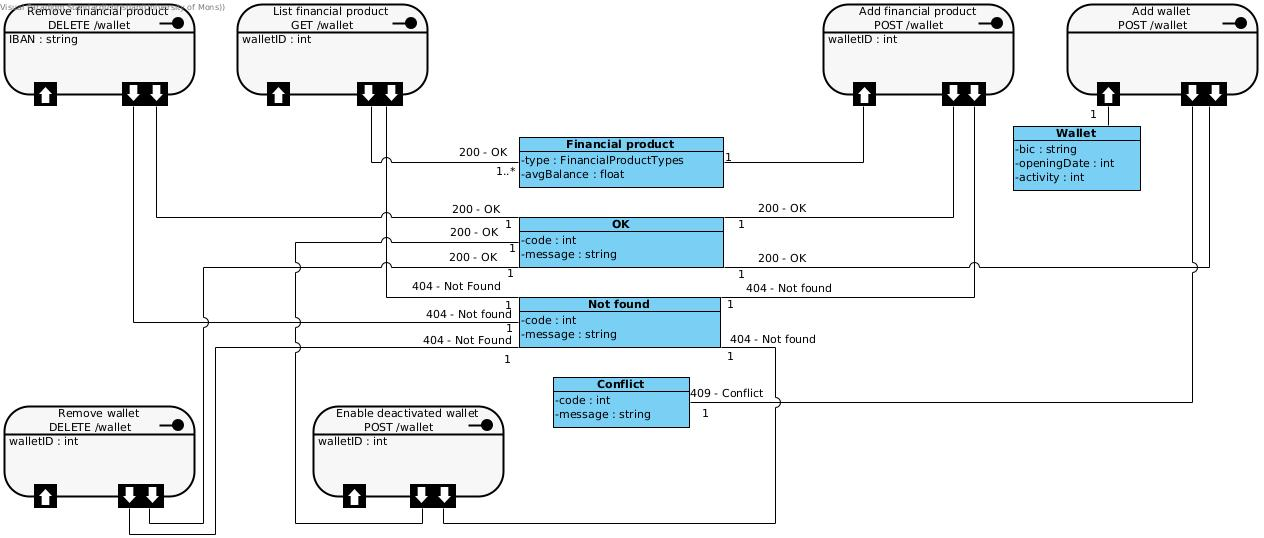
\includegraphics[scale=0.288]{ressources/photos_diagrammes/API/wallet.jpg}
    \caption{API de l'endpoint /wallet}
\end{figure}
\textit{\\wallet} permet d'intéragir avec les wallet et une partie de leur contenu (lister le contenu ou y ajouter un produit financier).

\begin{figure}[H]
    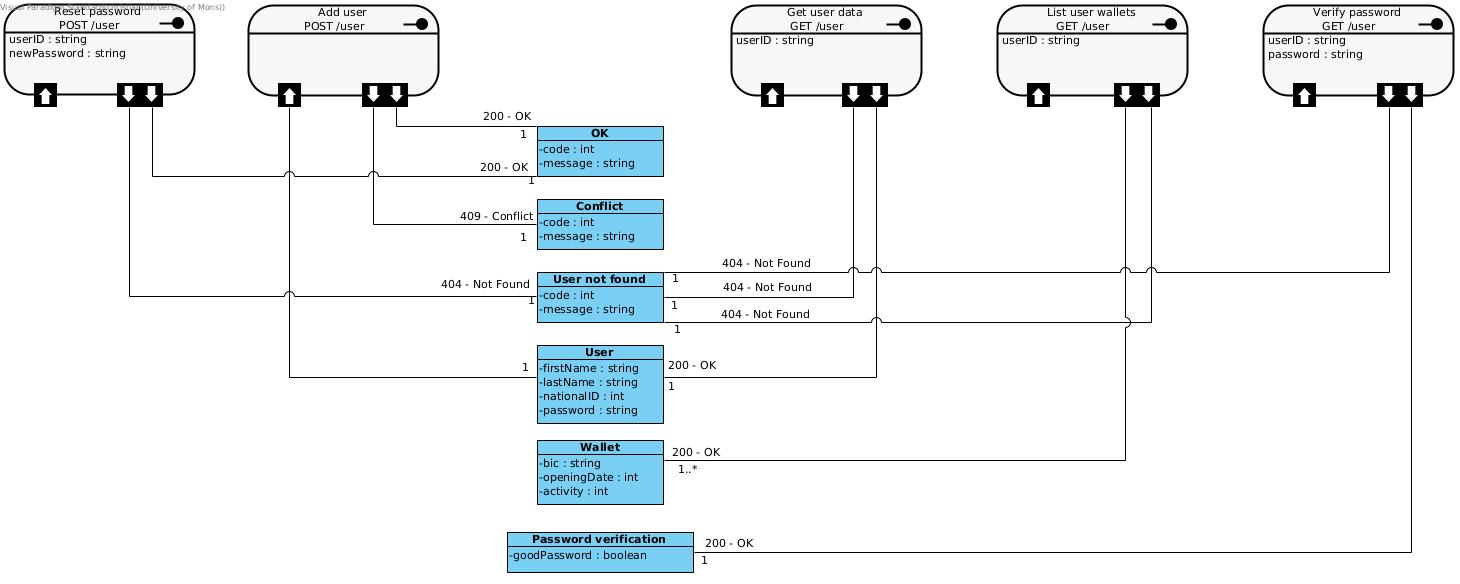
\includegraphics[scale=0.26]{ressources/photos_diagrammes/API/user.jpg}
    \caption{API de l'endpoint /user}
\end{figure}
\textit{\\user} permet d'intéragir avec les données d'un utilisateur, de lister ses wallets et de l'authentifier grâce à Verify password. La façon dont nous vérifions le mot de passe est à corriger car elle n'est pas sécurisée, le mot de passe est envoyé directement à l'API dans l'URI ce qui est vulnérable à une attaque du type "man in the middle" si une personne arrive à intercepter les requêtes. Même problème pour Reset password.

\begin{figure}[H]
    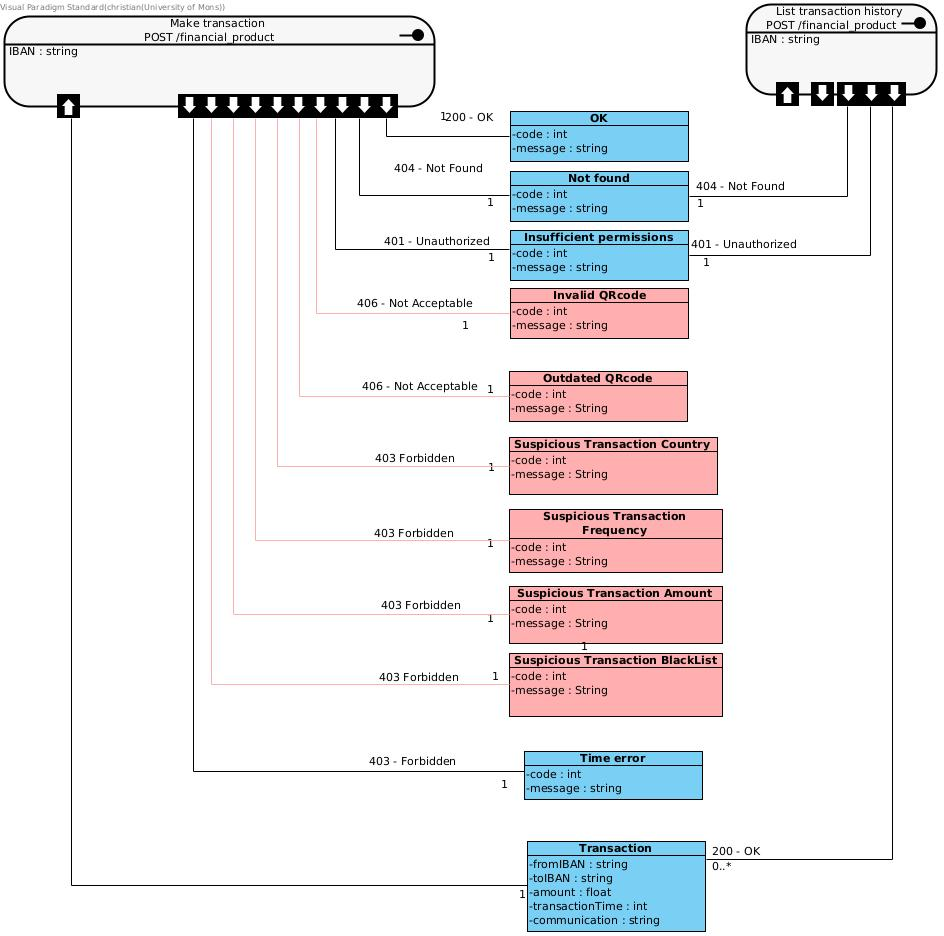
\includegraphics[scale=0.44]{ressources/photos_diagrammes/API/financial_product.jpg}
    \caption{API de l'endpoint /financial\_product}
\end{figure}
\textit{\\financial\_product} intéragit directement avec le contenu des produits financiers permettant de faire des transactions ou de voir l'historique. Nous avons essayé d'intégrer un certain degré de sécurité en utilisant un système de permission, il n'est pas visible sur le schéma mais on peut tout de même voir que l'API est capable de renvoyer le code d'erreur 401 - Unauthorized. \\
Nous pouvons aussi observer que Make transaction peut renvoyer une erreur 403 - Forbidden, dans notre cas elle est exclusivement utilisée pour signaler que le temps demandé pour effectuer la transaction n'est pas bon. Il doit être soit à 0 pour dire que la transaction doit être faite immédiatement ou sur une valeur dans le futur pour indiquer le temps auquel la transaction doit être faite. (nous utilisons UNIX time)

\newpage

\end{document}
